\chapter{Evaluation}
\label{chap:evaluation}

This chapter presents the evaluation of the selected alternatives, which are the combination of native Android and iOS, Apache Cordova and Motorola Rhodes. First, the weights of the evaluation criteria are calculated (Section \ref{sec:ev:crit}). Second, the weights of the selected alternatives are calculated (Section \ref{sec:ev:alt}), and last, a cost-benefit analysis is performed (Section \ref{sec:ev:costben}).

\section{Weighting the evaluation criteria}
\label{sec:ev:crit}

The weights for the evaluation criteria are calculated from judgements given by a developer and a mobile architect at Capgemini (the same people that gave the interviews in \ref{sec:interviews}). The judgements are collected from a questionnaire containing all necessary pairwise comparisons (see Appendix \ref{app:questionnaire}). The developer and the architect do no necessarily share the same opinions about the evaluation criteria. Therefore, this evaluation covers these two perspectives separately as they could have a different ranking of the alternatives. 

The weights (elements of the priority vector) are calculated as follows. The children of every non-leaf node in the evaluation criteria tree (visualized in \fref{fig:criteriatree}), are compared in pairs. For instance, the root node has three children, resulting in three pairwise comparisons: portability vs. application experience, application experience vs. productivity, and productivity vs. portability. The relative importance of two criteria is scored using Saaty's fundamental scale \cite{Saaty:1980, Saaty:1990} (see \tref{tab:ahp-scale}). For instance, if the architect strongly favours productivity over portability, a $5$ is written in the comparison matrix for the element productivity vs. portability (see \tref{tab:l1}). From this matrix, the principal right eigenvector is calculated and normalized\footnote{In AHP, a vector is normalized by dividing its elements by their sum.}. The consistency index is calculated from the eigenvector. More information about AHP can be found in Section \ref{sec:ahp}. Finally, the actual weight of every node is calculated as the product of all nodes that make up the path from the root node to that particular node.  

The following sections discuss the gathered judgements of the evaluation criteria.

\begin{figure}[h!]
    \centering
    \begin{sideways}
    \pstree[nodesep=3pt, thistreenodesize=1pt, thistreefit=loose]{\Tdot}{%
        \pstree[thistreenodesize=10pt]{\TR{\parbox{2cm}{\centering Portability}}}{%
            \TR{\parbox{2cm}{\centering Platform\\support}}
            \TR{\parbox{2cm}{\centering Toolset\\reuse}}
            \TR{\parbox{2cm}{\centering Code\\reuse}}
        }
        \pstree[thistreenodesize=20pt]{\TR{\parbox{2cm}{\centering Application\\Experience}}}{%
            \pstree[thistreenodesize=15pt]{\TR{\parbox{2cm}{\centering Native\\Integration}}}{%
                \TR{\parbox{2cm}{\centering Access to\\hardware}}
                \TR{\parbox{2cm}{\centering Platform-\\specific\\services}}
            }                    
            \pstree[thistreenodesize=10pt]{\TR{\parbox{2cm}{\centering UI\\capabilities}}}{%
                \TR{\parbox{2cm}{\centering Native\\L\&F}}
                \TR{\parbox{2cm}{\centering Element\\capabilities}}
            }                    
            \TR{\parbox{2cm}{\centering Performance}}
        }
        \pstree[thistreenodesize=10pt]{\TR{\parbox{2cm}{\centering Productivity}}}{%
            \TR{\parbox{2cm}{\centering Skill\\reuse}}
            \TR{\parbox{2cm}{\centering Tooling}}
            \TR{\parbox{2cm}{\centering Testing}}
        }
    }
    \end{sideways}
    \caption{The evaluation criteria, organized in a tree}
    \label{fig:criteriatree}
\end{figure}

\subsection{Top-level evaluation criteria}

The tree is decomposed into three top-level evaluation criteria: ``portability'', ``application experience'', and ``productivity''. The weight distribution for these criteria, presented in \tref{tab:portability}, is similar for both the architect and developer. There is, however, a large inconsistency in the judgement of the architect ($CR > 0.1$). In spite of the high inconsistency, the judgements are accepted because no new judgements could be gathered in time. Preferably, new judgements should be gathered until the consistency is satisfiable. 

\begin{table}[h!]
    \centering
    \begin{tabular}{lcccl}
        \hline
        \textbf{Architect}     & Portability & App. Experience & Productivity & Priority vector \\ 
        \hline
        Portability            & $1$         & $1/3$           & $1/5$        & $0.1047$        \\
        App. Experience        & $3$         & $1$             & $5$          & $0.6370$        \\
        Productivity           & $5$         & $1/5$           & $1$          & $0.2583$        \\
        \hline
        \multicolumn{5}{r}{$\lambda_{max} = 3.5206$, $CI = 0.2603$, $RI = 0.58$, $CR = 0.4488$} \\
        \hline
    \end{tabular}
    \\\vspace{1em}
    \begin{tabular}{lcccl}
        \hline
        \textbf{Developer}     & Portability & App. Experience & Productivity & Priority vector \\ 
        \hline
        Portability            & $1$         & $1/7$           & $1/5$        & $0.0719$        \\
        App. Experience        & $7$         & $1$             & $3$          & $0.6491$        \\
        Productivity           & $5$         & $1/3$           & $1$          & $0.2790$        \\
        \hline
        \multicolumn{5}{r}{$\lambda_{max} = 3.0649$, $CI = 0.0324$, $RI = 0.58$, $CR = 0.0559$} \\
        \hline
    \end{tabular}
    \caption{Pairwise comparison matrix for the top level of the decision tree.}
    \label{tab:l1}
\end{table}

\subsection{Portability}

The first top-level evaluation criterion, ``portability'', is decomposed into ``platform support'', ``toolset reuse'', and ``code reuse'' and the judgements of the developer and architect are illustrated in \tref{tab:portability}. Here, the differences between the developer and architect are a bit more pronounced but again, high consistency is observed in the architect's judgement. However, no better judgements were available. 

\begin{table}[h!]
    \centering
    \begin{tabular}{lcccl}
        \hline
        \textbf{Architect}     & Platform support & Toolset reuse & Code reuse & Priority vector \\ 
        \hline
        Platform support       & $1$            & $1/3$         & $1/7$      & $0.0918$          \\
        Toolset reuse          & $3$            & $1$           & $5$        & $0.6248$          \\
        Code reuse             & $7$            & $1/5$         & $1$        & $0.2834$          \\
        \hline
        \multicolumn{5}{r}{$\lambda_{max} = 3.7089$, $CI = 0.2545$, $RI = 0.58$, $CR = 0.6112$}  \\
        \hline
    \end{tabular}
    \\\vspace{1em}
    \begin{tabular}{lcccl}
        \hline
        \textbf{Developer}     & Platform support & Toolset reuse & Code reuse & Priority vector \\ 
        \hline
        Platform support         & $1$            & $1/5$         & $1/5$      & $0.0909\ldots$  \\
        Toolset reuse          & $5$            & $1$           & $1$        & $0.4545\ldots$  \\
        Code reuse             & $5$            & $1$           & $1$        & $0.4545\ldots$  \\
        \hline
        \multicolumn{5}{r}{$\lambda_{max} = 3$, $CI = 0$, $RI = 0.58$, $CR = 0$}               \\
        \hline
    \end{tabular}
    \caption{Pairwise comparison matrix for the category ``portability''.}
    \label{tab:portability}
\end{table}

\subsection{Application Experience}

The second top-level criterion, ``application experience'', is decomposed into ``native integration'', ``user interface capabilities'', and ``performance''. The gathered judgements from both developer and architect are listed in \tref{tab:ae}. Here, the differences are also pronounced. While the developer mainly focusses on performance, the architect prefers a mix of native integration and performance. Again, high inconsistency is noted in the architect's judgement.

\begin{table}[h!]
    \centering
    \begin{tabular}{lcccl}
        \hline
        \textbf{Architect}     & Native int. & UI capabilities & Performance & Priority vector \\ 
        \hline
        Native int.            & $1$         & $1$             & $3$         & $0.4600$        \\
        UI capabilities        & $1$         & $1$             & $1/3$       & $0.2211$        \\
        Performance            & $1/3$       & $3$             & $1$         & $0.3189$        \\
        \hline
        \multicolumn{5}{r}{$\lambda_{max} = 3.5608$, $CI = 0.2804$, $RI = 0.58$, $CR = 0.4835$}\\
        \hline
    \end{tabular}
    \\\vspace{1em}
    \begin{tabular}{lcccl}
        \hline
        \textbf{Developer}     & Native int. & UI capabilities & Performance & Priority vector \\ 
        \hline
        Native int.            & $1$         & $1$             & $1/5$       & $0.1428$        \\
        UI capabilities        & $1$         & $1$             & $1/5$       & $0.1428$        \\
        Performance            & $5$         & $5$             & $1$         & $0.7142$        \\
        \hline
        \multicolumn{5}{r}{$\lambda_{max} = 3$, $CI = 0$, $RI = 0.58$, $CR = 0$}               \\
        \hline
    \end{tabular}
    \caption{Pairwise comparison matrix for the category ``Application Experience''.}
    \label{tab:ae}
\end{table}

The criterion ``native integration'' is further broken down into ``access to hardware'' and ``platform-specific services''. Here, the developer and architect have clearly different opinions, as is visible in \tref{tab:ni}. Because there are only two subcriteria, there cannot be any inconsistency. 

\begin{table}[h!]
    \centering
    \begin{tabular}{lccl}
        \hline
        \textbf{Architect}     & Access to HW & Platform-specific svc. & Priority vector \\
        \hline
        Access to HW           & $1$          & $1/3$                  & $0.2500$        \\
        Platform-specific svc. & $3$          & $1$                    & $0.7500$        \\
        \hline
        \multicolumn{4}{r}{$\lambda_{max} = 2$, $CI = 0$, $RI = 0$, $CR = 0$}            \\
        \hline
    \end{tabular}
    \\\vspace{1em}
    \begin{tabular}{lccl}
        \hline
        \textbf{Developer}     & Access to HW & Platform-specific svc. & Priority vector \\
        \hline
        Access to HW           & $1$          & $5$                    & $0.8333\ldots$  \\
        Platform-specific svc. & $1/5$        & $1$                    & $0.1666\ldots$  \\
        \hline
        \multicolumn{4}{r}{$\lambda_{max} = 2$, $CI = 0$, $RI = 0$, $CR = 0$}            \\
        \hline
    \end{tabular}
    \caption{Pairwise comparison matrix for the category ``Native integration'' within the category ``Application Experience''.}
    \label{tab:ni}
\end{table}

The criterion ``user interface capabilities'' is also divided into two subcriteria: ``native look \& feel'' and ``user interface element capabilities''. Also here, the developer and architect have opposing opinions which is shown in \tref{tab:ui}. The architect strongly prefers native look and feel over element capabilities while it is the other way round for the developer. This has been observed earlier in the interviews as well (see Section \ref{sec:interviews}). Again, there is no inconsistency because there are only two subcriteria.

\begin{table}[h!]
    \centering
    \begin{tabular}{lccl}
        \hline
        \textbf{Architect}  & Native L\& F & UI el. capabilities & Priority vector \\
        \hline
        Native L\& F        & $1$          & $5$                 & $0.8333\ldots$  \\
        UI el. capabilities & $1/5$        & $1$                 & $0.1666\ldots$  \\
        \hline
        \multicolumn{4}{r}{$\lambda_{max} = 2$, $CI = 0$, $RI = 0$, $CR = 0$}      \\
        \hline
    \end{tabular}
    \\\vspace{1em}
    \begin{tabular}{lccl}
        \hline
        \textbf{Developer}  & Native L\& F & UI el. capabilities & Priority vector \\
        \hline
        Native L\& F        & $1$          & $1/5$               & $0.1666\ldots$  \\
        UI el. capabilities & $5$          & $1$                 & $0.8333\ldots$  \\
        \hline
        \multicolumn{4}{r}{$\lambda_{max} = 2$, $CI = 0$, $RI = 0$, $CR = 0$}      \\
        \hline
    \end{tabular}
    \caption{Pairwise comparison matrix for the category ``UI capabilities'' within the category ``Application Experience''.}
    \label{tab:ui}
\end{table}

\subsection{Productivity}

The last top-level criterion ``productivity'' is decomposed into ``skill reuse'', ``tooling'', and ``testing''. Apart from small deviations in judgement, the focus is mainly on tooling and skill reuse as can be seen from \tref{tab:productivity}. Here, the inconsistency in the architect's judgement is still high but rather acceptable.

\begin{table}[h!]
    \centering
    \begin{tabular}{lcccl}
        \hline
        \textbf{Architect} & Skill reuse & Tooling & Testing & Priority vector \\
        \hline
        Skill reuse        & $1$         & $1/5$   & $3$     & $0.2021$        \\
        Tooling            & $5$         & $1$     & $5$     & $0.7007$        \\
        Testing            & $1/3$       & $1/5$   & $1$     & $0.0972$        \\
        \hline
        \multicolumn{5}{r}{$\lambda_{max} = 3.1356$, $CI = 0.0678$, $RI = 0.58$, $CR = 0.1169$}\\
        \hline
    \end{tabular}
    \\\vspace{1em}
    \begin{tabular}{lcccl}
        \hline
        \textbf{Developer} & Skill reuse & Tooling & Testing & Priority vector \\
        \hline
        Skill reuse        & $1$         & $1$     & $3$     & $0.4286$        \\
        Tooling            & $1$         & $1$     & $3$     & $0.4286$        \\
        Testing            & $1/3$       & $1/3$   & $1$     & $0.1428$        \\
        \hline
        \multicolumn{5}{r}{$\lambda_{max} = 3$, $CI = 0$, $RI = 0.58$, $CR = 0$}               \\
        \hline
    \end{tabular}
    \caption{Pairwise comparison matrix for the category ``Productivity''.}
    \label{tab:productivity}
\end{table}

\section{Evaluate the alternatives}
\label{sec:ev:alt}

In the subsections to follow, all alternatives are evaluated with respect to one criterion at a time. Every subsection gives a description of what is measured and how. Additionally, the description also illustrates what is taken into account for the evaluation, which scale is used and why. For every alternative, a rationale is provided for the judgement or attributed score.

For some criteria, there is no absolute scale available to measure that specific property. In that case, judgements based on pairwise comparison, as proposed by Saaty \cite{Saaty:1980}, are used in order to evaluate the alternatives. These judgements arise from the experience of developing the proof-of-concept application. In addition, some criteria deal with features that are not addressed in the proof-of-concept application. In that case, the evaluation is based on the information found in the documentation of the different tools. 

\TODO{Make sure every section clearly mentions these things...}

\subsection{Platform support}

As mentioned in Section \ref{sec:selection-criteria}, support for Android and iOS is a selection criterion. Hence, this criterion only covers additional platforms, in addition to Android and iOS. To reflect the value of each platform, every alternative is awarded the additional market share it can serve. In the end, these scores are normalized (the sum of scores is equal to 1). The market share numbers are taken from research by Gartner \citeGartner (see \fref{fig:smartphone-share}).

\paragraph{Android \& iOS} Native code for Android and iOS is useless on other platforms. Hence, the combination of Android and iOS cannot contribute to reaching additional market share.

\paragraph{Apache Cordova} From Cordova's platform support, it is safe to say that it supports the remainder of the mobile market. Cordova is therefore awarded the remaining 17\% of market share: 6\% for BlackBerry, 6\% for Symbian, 2\% for Windows Phone, 2\% for Bada and 1\% for the remainder of mobile platforms.

\paragraph{Motorola Rhodes} Rhodes only supports BlackBerry and Windows Phone for which it is awarded 8\% of market share: 6\% for BlackBerry and 2\% for Windows Phone. 

Applications that are built with the native SDK's can only be used on their intended platforms. Cordova and Rhodes can reach additional platforms, which is shown in \tref{tab:ps}. 

\begin{table}[h!]
    \centering
    \begin{tabular}{lcccl}
        \hline
        \textbf{Platform support} & Market share & Normalized weight \\
        \hline
        Android/iOS               & $0\%$        & $0$               \\
        Cordova                   & $17\%$       & $0.68$            \\
        Rhodes                    & $8\%$        & $0.32$            \\
        \hline
    \end{tabular}
    \caption{Evaluation of the alternatives with respect to ``platform support''.}
    \label{tab:ps}
\end{table}

\subsection{Toolset reuse}

This criterion describes the ability to reuse the development environment or parts thereof (1) for the development for both platforms and (2) when migrating to another cross-platform alternative. The evaluation is based on the recommended development environment setup for each alternative. Since there is no absolute scale available to measure this property, Saaty's fundamental scale (see \tref{tab:ahp-scale}) is used here.

\paragraph{Android \& iOS} All iOS development is done with the Xcode IDE, which is available on Mac OS X only. Every iOS developer must therefore own an Apple computer. For Android development, any operating system can be used in combination with the Android SDK and an Eclipse IDE for which a plugin, called Android Development Toolkit (ADT), is available. On the latest developer conference, Google also announced a new and freely available Android IDE, based on JetBrains' IntelliJ IDEA\footnote{IntelliJ IDEA is another Java IDE, comparable to Eclipse, \url{http://jetbrains.com/idea}}.

\paragraph{Apache Cordova} For HTML5 application development, any operating system with a web IDE or even a simple text editor is sufficient. However, packaging the Cordova application in its native shell requires the native SDK's or an online build service like PhoneGap Build. These online build services enable developers with Windows or Linux operating systems to develop applications for iOS. Unfortunately, this particular service cannot build additional plugins that are not part of the standard distribution. If a project makes use of custom plugins, the environment has the same requirements as that of the native SDK's. 

\paragraph{Motorola Rhodes} Development of Rhodes applications requires a Ruby installation and a Ruby IDE. A specially tailored Eclipse-based Ruby IDE, called RhoStudio, is distributed as part of RhoMobile. As with Cordova, packaging the app requires the native SDK or an online build service, like RhoHub. 

The development environments for Rhodes and Cordova are quite similar and are treated equally in the comparison for that reason. Android and iOS are treated as a whole and because of Apple's strict requirements, it is more limited than Rhodes and Cordova. But, if the development environment is based on OS X, then there are no notable differences. This rationale is summarized in \tref{tab:tr}.

\begin{table}[h!]
    \centering
    \begin{tabular}{lcccl}
        \hline
        \textbf{Toolset reuse} & Android/iOS & Cordova & Rhodes & Priority vector \\
        \hline
        Android/iOS            & $1$         & $1/3$   & $1/3$  & $0.1428$        \\
        Cordova                & $3$         & $1$     & $1$    & $0.4286$        \\
        Rhodes                 & $3$         & $1$     & $1$    & $0.4286$        \\
        \hline
        \multicolumn{5}{r}{$\lambda_{max} = 3$, $CI = 0$, $RI = 0.58$, $CR = 0$}  \\
        \hline
    \end{tabular}
    \caption{Evaluation of the alternatives with respect to ``toolset reuse''.}
    \label{tab:tr}
\end{table}

\subsection{Code reuse}
\label{sec:cr}

This criterion measures the amount of code that can be reused when migrating to another platform. For this criterion, the amount of portable code is expressed as an estimated percentage of the total amount of application code. Native extensions (through pluggable architectures) are not taken into account as they are not part of the application logic. They are in fact reusable software components that can be coded once and used many times afterwards. 

\paragraph{Android \& iOS} As mentioned before, native code for Android and iOS is useless on other platforms but native Android code is also useless on iOS and vice versa. Hence, code reuse on Android and iOS is 0\%.

\paragraph{Apache Cordova} Cordova wraps mobile web applications. Hence, all (or 100\%) of the application code can be easily shared across platforms. Cordova has a pluggable architecture but --- as mentioned in the description --- this is not taken into account in this discussion.

Note that a substantial amount of code (or potentially all code) can be reused on other (non-mobile) platforms. Cordova applications only use client-side programming languages and the API's match existing HTML5 specifications. Therefore, these applications can be easily ported to other, non-mobile platforms. However, non-mobile platforms are out of scope for this evaluation.

\paragraph{Motorola Rhodes} The application logic of Rhodes applications can be fully shared across platforms as well. Hence, code reuse is also 100\%. Rhodes also has plugin system but, these are not taken into account. In contrast to Cordova, Rhodes applications are based on the Rhodes MVC framework which makes it hard (or even impossible) to deploy them outside a Rhodes environment.

The native code for Android and iOS cannot be reused across platforms whereas all the code is reused in Cordova and Rhodes application. This is shown in \tref{tab:cr}. 

\begin{table}[h!]
    \centering
    \begin{tabular}{lcccl}
        \hline
        \textbf{Toolset reuse} & Code reuse & Priority vector \\
        \hline
        Android/iOS            & $0\%$       & $0$            \\
        Cordova                & $100\%$     & $0.5000$       \\
        Rhodes                 & $100\%$     & $0.5000$       \\
        \hline
    \end{tabular}
    \caption{Evaluation of the alternatives with respect to ``code reuse''.}
    \label{tab:cr}
\end{table}

\subsection{Access to hardware}

This criterion measures the ability to integrate with the device's hardware. The availability of device API's (sensor API's, output API's, and communication API's) of every alternative is compared side by side. An alternative can either provide full support, partial support or no support at all. If an additional plugin system is present, the alternative could provide the same levels of support through a plugin. Note that most of these API's are not used in the proof-of-concept application. Therefore, this comparison is mostly based on the documentation of the alternatives.

\paragraph{Android \& iOS} Android provides full access to the device but that does not imply that all these device features are available on a particular device. Apple's iDevices have less device features but provide full support for those that are present.

\paragraph{Apache Cordova} Cordova tries to promote the web as a first-class platform for mobile applications. ``The ultimate purpose of \emph{Cordova} is to cease to exist'' \cite{LeRoux:2012}. When HTML5 will be fully supported on all mobile browsers, Cordova will no longer be needed. Therefore, Cordova API's mostly match the HTML5 specification and do not provide support for all the sensors and communication because they are simply not part of the specification. However, Cordova comes with an elaborate plugin system which can be used to reach the same level of integration as native Android and iOS. 

\paragraph{Motorola Rhodes} Rhodes has a unified sensors API on which one can listen for events coming from all types of sensors if they are present. Rhodes lacks a VideoCapture feature on all platforms and a MediaPlayer on iOS out of the box but these can be implemented using the plugin system. 

\begin{table}[h!]
    \centering
    \begin{tabular}{lcccc}
        \hline
        API                       & Android        & iOS                  & Cordova    & Rhodes                   \\
        \hline          
        Accelerometer             & \checkmark     & \checkmark           & \checkmark        & \checkmark        \\
        Geolocation               & \checkmark     & \checkmark           & \checkmark        & \checkmark        \\
        Gyroscope                 & \checkmark     & \checkmark           & full w/ plugin    & \checkmark        \\
        Light                     & \checkmark     & \checkmark           & full w/ plugin    & \checkmark        \\
        Magnetic Field            & \checkmark     & \checkmark           & \checkmark        & \checkmark        \\
        Pressure                  & \checkmark     & --                   & partial w/ plugin & partial           \\
        Proximity                 & \checkmark     & \checkmark           & full w/ plugin    & \checkmark        \\
        Relative Humidity         & \checkmark     & --                   & partial w/ plugin & partial           \\
        Temperature               & \checkmark     & --                   & partial w/ plugin & partial           \\
        Microphone                & \checkmark     & \checkmark           & \checkmark        & \checkmark        \\
        Camera                    & \checkmark     & \checkmark           & \checkmark        & partial           \\
        Hardware buttons          & \checkmark     & --                   & partial           & partial           \\
        Vibration Motor           & \checkmark     & \checkmark           & \checkmark        & partial           \\
        Speaker                   & \checkmark     & \checkmark           & \checkmark        & partial           \\       
        System information        & \checkmark     & \checkmark           & \checkmark        & \checkmark        \\
        File System               & \checkmark     & \checkmark           & \checkmark        & \checkmark        \\
        Contacts                  & \checkmark     & \checkmark           & \checkmark        & \checkmark        \\
        Bluetooth                 & \checkmark     & \checkmark           & full w/ plugin    & \checkmark        \\
        NFC                       & \checkmark     & --                   & partial w/ plugin & partial w/ plugin \\
        Wi-Fi Direct              & \checkmark     & --                   & partial w/ plugin & partial w/ plugin \\
        USB / Accessory           & \checkmark     & \checkmark           & full w/ plugin    & full w/ plugin    \\
        \hline      
        Full support              & \multicolumn{2}{c}{Combined: $15/21$} & $10/21$           & $11/21$           \\
        Partial support           & \multicolumn{2}{c}{Combined:  $6/21$} &  $1/21$           &  $7/21$           \\
        Full support w/ plugin    & \multicolumn{2}{c}{Combined:  $0/21$} &  $5/21$           &  $1/21$           \\
        Partial support w/ plugin & \multicolumn{2}{c}{Combined:  $0/21$} &  $5/21$           &  $2/21$           \\
        \hline
        Total                     & \multicolumn{2}{c}{Combined: $21/21$} &  $21/21$          & $21/21$           \\
        \hline
    \end{tabular}
    \caption{Evaluation of the alternatives with respect to ``access to hardware''.}
    \label{tab:apis}
\end{table}

From \tref{tab:apis}, it is clear that all device features can be integrated with, independent of the alternative used. If the alternative does not support a current feature out of the box, it can be reached trough a plugin. This requires some additional native coding but the plugin can be reused. Therefore, Cordova and Rhodes are only mildly penalized in \tref{tab:hwaccess}.

\begin{table}[h!]
    \centering
    \begin{tabular}{lcccl}
        \hline
        \textbf{Access to hardware} & Android/iOS & Cordova & Rhodes & Priority vector \\
        \hline
        Android/iOS          & $1$         & $3$     & $3$   & $0.6000$        \\
        Cordova              & $1/3$       & $1$     & $1$   & $0.2000$        \\
        Rhodes               & $1/3$       & $1$     & $1$   & $0.2000$        \\
        \hline
        \multicolumn{5}{r}{$\lambda_{max} = 3$, $CI = 0$, $RI = 0.58$, $CR = 0$}\\
        \hline
    \end{tabular}
    \caption{Evaluation of the alternatives with respect to ``access to hardware''}
    \label{tab:hwaccess}
\end{table}

\subsection{Integration with platform-specific services}

This criterion measures the ability to integrate with platform-specific services, like push notifications. The proof-of-concept application does not require this kind of integration and thus this evaluation is based on the documentation. Because there is no absolute scale to quantify this property, the evaluation is also based on judgements.

\paragraph{Android \& iOS} Platform-specific services are part of the native SDK's. Therefore, this kind of integration is easily implemented in native applications.

\paragraph{Apache Cordova} There are no API's for this kind of integration in the default distribution. Fortunately though, Cordova ships with an elaborate plugin-system which can be used to deal with it.

\paragraph{Motorola Rhodes} In Rhodes, there are no API's for this integration either. However, Rhodes also has a plugin system which can make this integration possible. 

Integrating with platform-specific services is obviously more easy when programming natively. However, the other alternatives can use their plugin system to provide this integration. Since plugins can be reused easily, this is only deemed to be a minor disadvantage which is visible in the judgements, listed in \tref{tab:pss}. 

\begin{table}[h!]
    \centering
    \begin{tabular}{lcccl}
        \hline
        \textbf{Platform-specific services} & Android/iOS & Cordova & Rhodes & Priority vector \\
        \hline
        Android/iOS          & $1$         & $3$     & $3$   & $0.6000$        \\
        Cordova              & $1/3$       & $1$     & $1$   & $0.2000$        \\
        Rhodes               & $1/3$       & $1$     & $1$   & $0.2000$        \\
        \hline
        \multicolumn{5}{r}{$\lambda_{max} = 3$, $CI = 0$, $RI = 0.58$, $CR = 0$}\\
        \hline
    \end{tabular}
    \caption{Evaluation of the alternatives with respect to ``platform-specific services''}
    \label{tab:pss}
\end{table}

\subsection{Native Look \& Feel}

This criterion indicates whether or not an alternative is able to use native user interface elements. An application can either support the use of native user interface elements fully, partially or not at all. It needs no explaining that Android and iOS can use the native user interface elements.

\paragraph{Apache Cordova} The user interface of Cordova applications is built with HTML5, CSS and JavaScript and there is no possibility to use native user interface elements for it. However, numerous attempts are made to recreate the native look \& feel on top of HTML (like KendoUI, Moobile, etc.). Unfortunately, these projects need a lot of additional code to mimic the behaviour of native interface elements which influences the overall performance of the application in an adverse way.

\paragraph{Motorola Rhodes} The user interface of Rhodes applications is also built with HTML and consequently cannot deliver the native look \& feel to the end user.

Despite the efforts of many projects to mock the native look \& feel in web applications, it remains a privilege of Android and iOS. Hence, Android and iOS clearly score better compared to Cordova and Rhodes, as is illustrated in \tref{tab:nlf}.

\begin{table}[h!]
    \centering
    \begin{tabular}{lcl}
        \hline
        \textbf{Native Look \& Feel} & Native L\&F & Priority vector \\
        \hline
        Android/iOS                  & Yes         & $1$  \\
        Cordova                      & No          & $0$  \\
        Rhodes                       & No          & $0$  \\
        \hline
    \end{tabular}
    \caption{Evaluation of the alternatives with respect to ``Native look \& feel''.}
    \label{tab:nlf}
\end{table}

\subsection{UI element capabilities}

This criterion measures an alternative's potential to present a rich user interface. Both Cordova and Rhodes rely on HTML for their user interface. Therefore, the evaluation is based on a comparison of the native UI elements with their HTML5 counterparts. In the proof-of-concept application, an additional UI framework, called Bootstrap, was used to create a rich user interface. In this evaluation, alternatives for the typical native user interface elements are searched in the HTML5 specification and the Bootstrap framework.

\paragraph{Android \& iOS} Android and iOS both have an elaborate portfolio of rich user interface elements. iOS lacks some basic form elements like radio buttons and checkboxes but these can be easily replaced with pickers and switches respectively.

\paragraph{Apache Cordova} Cordova applications are mobile web applications that are wrapped in a single webview. Hence, only HTML5 can be used to create the user interface. An application could be comprised of multiple pages or it could be comprised of a single page, in which case it is called  a single-page application. The former approach requires page reloads, which feels unnatural in a mobile app (compared to native apps) whereas the latter approach can make the hybrid app behave more like a native app. 

The Cordova proof-of-concept application is implemented as a single-page application with AngularJS\footnote{\url{http://angularjs.org}}. This framework drastically improves productivity by reducing the required lines of code through declarative programming and bidirectional bindings between view and model. 

\paragraph{Motorola Rhodes} Rhodes also relies on HTML for its user interface. In contrast to Cordova, Rhodes is actually a complete web server with an MVC framework on top. Every request is handled locally by a controller action and the result is served in a webview. Developers can still choose to create single-page applications but device integration has to be realized through AJAX\footnote{Asynchronous JavaScript and XML} calls, which requires extra work. The proof-of-concept application is implemented as a multi-page application because this is the default way to develop applications with Rhodes.

HTML only offers basic user interface building blocks. However, with these blocks, one can create a very rich user interface, e.g. by using \html{a}'s, \html{div}'s, list elements and styling one can create create powerful navigation bars. The use of an additional user interface framework like Bootstrap can be a great help in this area. In the end, all alternatives have a more or less equally rich user interface, which is indicated in \tref{tab:uiec}.

\begin{table}[h!]
    \centering
    \begin{tabular}{llll}
        \hline
        Android         & iOS              & HTML5                          & Bootstrap 3             \\
        \hline
        ActionBar       & UINavigationBar  & --                             & \html{navbar} class     \\
        Split ActionBar & UIToolbar        & --                             & \html{navbar} class     \\
        Tabs            & UITabBar         & --                             & \html{nav-tabs} class   \\
        ListView        & UITableView      & --                             & \html{list-group} class \\
        GridList        & UICollectionView & --                             & Grid system             \\            
        ScrollView      & UIScrollView     & by default                     & --                      \\
        Spinner         & --               & \html{<select></select>}       & \html{dropdown} class   \\
        Picker          & UIPickerView     & \html{<select></select>}       & \html{modal} class      \\
        DatePicker      & UIDatePicker     & \html{<input type="date">}     & --                      \\
        Button          & UIButton         & \html{<button></button>}       & \html{btn} class        \\
        Text field      & UITextField      & \html{<input type="...">}      & --                      \\
        Slider          & UISlider         & \html{<input type="range">}    & --                      \\
        Progress bar    & UIProgressBar    & \html{<progress>}              & \html{progress} class   \\
        Options Menu    & UIActionSheet    & --                             & --                      \\
        Checkbox        & --               & \html{<input type="checkbox">} & --                      \\
        Radio           & --               & \html{<input type="radio">}    & --                      \\
        On/off switch   & UISwitch         & --                             & \html{btn-group} class  \\
        Dialog          & UIDialog         & --                             & \html{modal} class      \\
        Alert           & UIAlertView      & \html{alert(string)}           & --                      \\
        Popup           & --               & --                             & \html{modal} class      \\
        Toast           & --               & --                             & \html{alert} class      \\
        TextView        & UILabel          & any text element               & --                      \\
        MapView         & MKMapView        & --                             & --                      \\
        --              & Popover (iPad)   & --                             & \html{popover} script   \\
        Master-Detail   & SplitView (iPad) & --                             & Grid System             \\
        WebView         & UIWebView        & \html{<iframe>}                & --                      \\
        \hline
        \multicolumn{2}{c}{Android \& iOS combined: $26/26$} & \multicolumn{2}{c}{HTML5 \& Bootstrap combined: $24/26$}                 \\
        \hline
    \end{tabular}
    \caption{Evaluation of the alternatives with respect to ``UI element capabilities''.}
    \label{tab:uiec}
\end{table}

\subsection{Performance}

The performance criterion measures the responsiveness of the user interface and the application in general. Responsiveness in this case does not mean the ability to reflow UI elements to fit other screen sizes, responsiveness in this case represents the time it takes an application to respond to a trigger, like pushing a button.

Comparing the performance of these alternatives is hard because their architectures are completely different. For web applications, page load times could be a viable metric. However, only the Rhodes application uses page loads. There is no notion of page loads in native applications and the Cordova application is implemented as a single-page application. Hence, no absolute scale is available and the alternatives are evaluated based on judgement. The analytic hierarchy process can deal with inconsistency as long as the consistency ratio is low, i.e equal or below 10\%. In that case, the judgements are accepted. 

Every implementation of the proof-of-concept application is tested on four devices:
\begin{itemize}
    \item \textbf{HTC Wildfire S} An entry-level smartphone, released in May 2011 and running Android 2.3.5 on a single core 600\,MHz ARMv6 processor. It has 512\,MB of RAM and a 3.2-inch display with a 320 by 480 pixel resolution (180\,ppi).
    \item \textbf{HTC Flyer} An entry-level tablet, also released in May 2011 and running Android 3.2.2 on a single core 1.5\,GHz ARMv7 processor. It has 1024\,MB of RAM and a 7.0-inch display with a 600 by 1024 pixel resolution (170\,ppi).
    \item \textbf{LG/Google Nexus 4} A high-end smartphone, released in November 2012 and running Android 4.2.2 on a quad core 1.5\,GHz ARMv7 processor. It has 2048\,MB of RAM and a 4.7-inch display with a 768 by 1280 pixel resolution (318\,ppi).
    \item \textbf{iPhone 3GS} A smartphone, released in June 2009 and running iOS 6.1.3 on a single core 600\,MHz ARMv6 processor. It has 256\,MB of RAM and a 3.5-inch display with a 320 by 480 pixel resolution (165\,ppi).
    \item \textbf{iPad} A tablet, released in 2010 and running iOS 5.1.1 on a single core 1\,GHz ARMv7 processor. It has 256\,MB of RAM and a 9.7-inch display with a 768 by 1024 pixel resolution (132\,ppi).
\end{itemize}

\paragraph{Android \& iOS} The native SDK's are best placed to take advantage of the device capabilities. Therefore, native applications always perform the best, provided they are well-designed.

\paragraph{Apache Cordova} Cordova wraps web applications. Hence, the performance of its applications greatly depends on the performance of the browser on the device. On older smartphones, the performance of the browser is often seriously lacking. The use of a single-page application solves this issue in a way, but the performance drop is still notable.

\paragraph{Motorola Rhodes} A Rhodes application also relies on the native browser to display its user interface. The difference with Cordova is that Rhodes uses a local ruby web server to serve multi-page applications. The performance of the local web server is disappointing, resulting in utterly slow page loads (of up to 30 seconds for a single load on the slowest devices and 7 seconds on the fastest device).

The judgements for this evaluation are listed in \tref{tab:performance}. The consistency ratio is rather high but still acceptable.

\begin{table}[h!]
    \centering
    \begin{tabular}{lcccl}
        \hline
        \textbf{Performance} & Android/iOS & Cordova & Rhodes & Priority vector \\
        \hline
        Android/iOS          & $1$         & $5$     & $9$    & $0.7352$        \\
        Cordova              & $1/5$       & $1$     & $5$    & $0.2067$        \\
        Rhodes               & $1/9$       & $1/5$   & $1$    & $0.0581$        \\
        \hline
        \multicolumn{5}{r}{$\lambda_{max} = 3$, $CI = 0.0585$, $RI = 0.58$, $CR = 0.10$}\\
        \hline
    \end{tabular}
    \caption{Evaluation of the alternatives with respect to ``Performance''.}
    \label{tab:performance}
\end{table}

\subsection{Skill reuse}

This criterion expresses the ability to reuse skills from another field of expertise to develop mobile applications. This allows for better resource management. For this criterion, it is assumed that the organization has got experience with Java and web development (because these are the areas of expertise at Capgemini). 

\paragraph{Android \& iOS} For organizations that already have expertise with Java development, the entry barrier for adding Android to the portfolio is rather low, since Android is based on Java. Adding iOS from that perspective is less straightforward, because Objective-C is a new programming language.

\paragraph{Apache Cordova} In order to develop Cordova applications, one needs to know the web. Since the web already belongs to the organization's expertise, this skill can be reused quite easily but developers will probably have to invest in their JavaScript skills. When custom plugins are needed, the scenario of native Android and iOS holds.

\paragraph{Motorola Rhodes} For Rhodes applications, organizations can reuse their skills for creating the user interface. However, the application logic entirely written in Ruby, which is a new programming language for the organization.

The native SDK's and Rhodes are similar because one needs to learn a new language for either of both. For the development of Cordova application, no notable new skills are required, explaining the scores listed in \tref{tab:sr}.

\begin{table}[h!]
    \centering
    \begin{tabular}{lcccl}
        \hline
        \textbf{Skill reuse} & Android/iOS & Cordova & Rhodes & Priority vector \\
        \hline
        Android/iOS          & $1$         & $1/5$   & $1$    & $0.1428$        \\
        Cordova              & $5$         & $1$     & $5$    & $0.7144$        \\
        Rhodes               & $1$         & $1/5$   & $1$    & $0.1428$        \\
        \hline
        \multicolumn{5}{r}{$\lambda_{max} = 3$, $CI = 0$, $RI = 0.58$, $CR = 0$}\\
        \hline
    \end{tabular}
    \caption{Evaluation of the alternatives with respect to ``Skill reuse''.}
    \label{tab:sr}
\end{table}

\subsection{Tooling}

This criterion describes the overall quality of the supplied tools. This includes command-line interfaces, IDE's, emulators and others. Since there is no absolute scale available to measure the quality accurately, the alternatives are compared in pairs. Saaty's scale is used to express the scores that are based on the experience of developing the proof-of-concept application (see \tref{tab:ahp-scales}).

\paragraph{Android \& iOS} The restrictions on Apple development may seem obstructive at first but it also allows Apple to deliver a well integrated development environment. Everything a developer could possibly need is available in Xcode, right out of the box. For Android development, an Eclipse plugin is available which integrates all the functionality of the SDK with the IDE. 

\paragraph{Apache Cordova} Cordova does not ship with an elaborate IDE or special development tools. However, there are some tools that can ease the development of mobile web applications (WEINRE, Ripple emulator, etc.). Unfortunately, there is no integrated development environment. 

\paragraph{Motorola Rhodes} Rhodes ships with command-line interface for building the application. Sadly, this interface poorly integrates with the  Android Debug Bridge (ADB) and there is no option to transfer iOS applications to an iDevice. Instead, either Xcode, iTunes or Fruitstrap\footnote{Fruitstrap is a command-line script for transferring applications to an iDevice, \url{https://github.com/ghughes/fruitstrap}} is needed for the transfer. Next to the command-line tools, Rhodes also ships with an Eclipse-based IDE, called RhoStudio. However, this IDE could not be configured to make it work with the Rhodes SDK. 

The experience with the tools during the development of the proof-of-concept application are listed in \tref{tab:tooling}. The experience with Rhodes was awful and the experience with Cordova was a little less pleasant than with the tools for native Android and iOS. 

\begin{table}[h!]
    \centering
    \begin{tabular}{lcccl}
        \hline
        \textbf{Tooling} & Android/iOS & Cordova & Rhodes & Priority vector \\
        \hline
        Android/iOS      & $1$         & $3$     & $9$    & $0.6716$        \\
        Cordova          & $1/3$       & $1$     & $5$    & $0.2654$        \\
        Rhodes           & $1/9$       & $1/5$   & $1$    & $0.0629$        \\
        \hline
        \multicolumn{5}{r}{$\lambda_{max} = 3$, $CI = 0.0145$, $RI = 0.58$, $CR = 0.025$}\\
        \hline
    \end{tabular}
    \caption{Evaluation of the alternatives with respect to ``Tooling''.}
    \label{tab:tooling}
\end{table}

\subsection{Testing}

This criterion measures both the ability to (1) write tests, and (2) automate testing in a continuous integration environment. This criterion focusses mainly on unit testing and integration testing as these tests are most common. End-user testing is not taken into account for this criterion. Alternatives are evaluated using judgements because there is no absolute scale on which this property could be quantified. 

Continuous integration is actually not part of the scope for the proof-of-concept application. Nevertheless, since this is an important topic in a production environment, the basics are examined.

\paragraph{Android \& iOS} Android and iOS have built-in support for writing unit tests (1). Android is based on Java and consequently, the well-known JUnit framework can be used for writing tests. For iOS, a similar framework is readily available in Xcode for Objective-C. For automated testing in a continuous integration environment (2), there are a number of options available. Continuous integration testing for Android can be set up quite easily with Jenkins\footnote{Jenkins is a popular continuous integration server, \url{http://jenkins-ci.org}}, even headless\footnote{On a server without a user interface}. For iOS, there are a number of guides available describing how to set it up. However, Apple hardware is still required. Other options include a hosted continuous integration service.

\paragraph{Apache Cordova} For JavaScript, the Jasmine testing framework can be used to write tests (1). In combination with a test runner like Karma, these test can be automated in a continuous integration environment. Better yet, this framework allows to automate testing on the actual mobile devices.

\paragraph{Motorola Rhodes} Unit testing is also built-in into Rhodes. However, only few options seem to be available for automating testing in a continuous integration environment.

The judgements are summarized in \tref{tab:testing}. All alternatives have support for unit testing. In that perspective, they are all equal but Rhodes seems to be less suited for continuous integration when compared to the other alternatives. The other alternatives perform equally because seem to support the same features.

\begin{table}[h!]
    \centering
    \begin{tabular}{lcccl}
        \hline
        \textbf{Testing} & Android/iOS & Cordova & Rhodes & Priority vector \\
        \hline
        Android/iOS      & $1$         & $1$     & $3$    & $0.4286$ \\
        Cordova          & $1$         & $1$     & $3$    & $0.4286$ \\
        Rhodes           & $1/3$       & $1/3$   & $1$    & $0.1428$ \\
        \hline
        \multicolumn{5}{r}{$\lambda_{max} = 3$, $CI = 0$, $RI = 0.58$, $CR = 0$}\\
        \hline
    \end{tabular}
    \caption{Evaluation of the alternatives with respect to ``Testing''.}
    \label{tab:testing}
\end{table}

\section{Global verdict}

The weights of all alternatives with respect to the evaluation criteria is illustrated in \fref{fig:radar}. Now that the weights of both the criteria and alternatives are given, the total weight $a_j$ of every alternative $A_j$ is calculated as
\begin{gather*}
    a_j = \sum_{i = 0}^{m} c_i w_i \quad j = 1, \ldots, n
\end{gather*}
where $c_i$ is the weight of the criterion $C_i$ and $w_i$ is the weight of alternative $A_j$ with respect to criterion $C_i$. The total weights are calculated for both the architect and developer and are listed in \tref{tab:total:architect} and \tref{tab:total:developer} respectively. 

\begin{figure}
    \centering
    %\includegraphics[width=0.7\textwidth]{figs/radar.pdf}
    \caption{A radar graph, visualizing the weights of all alternatives}
    \label{fig:radar}
\end{figure}

\begin{table}[h]
    \centering
    \begin{tabular}{lcccc}
        \hline
        \textbf{Architect}         & $c_i$    & $c_i w_{Android/iOS}$ & $c_i w_{Cordova}$  & $c_i w_{Rhodes}$ \\
        \hline
        Platform support           & $0.0096$ & $0.0000$              & $0.0065$           & $0.0031$     \\
        Toolset reuse              & $0.0654$ & $0.0093$              & $0.0280$           & $0.0280$     \\
        Code reuse                 & $0.0297$ & $0.0000$              & $0.0148$           & $0.0148$     \\
        Access to hardware         & $0.0733$ & $0.0300$              & $0.0175$           & $0.0258$     \\
        Platform-specific services & $0.2198$ & $0.1831$              & $0.0366$           & $0.0000$     \\
        Native Look \& Feel        & $0.1174$ & $0.1174$              & $0.0000$           & $0.0000$     \\
        UI element capabilities    & $0.0235$ & $0.0110$              & $0.0062$           & $0.0062$     \\
        Performance                & $0.2031$ & $0.1493$              & $0.0420$           & $0.0118$     \\
        Skill reuse                & $0.0522$ & $0.0135$              & $0.0333$           & $0.0055$     \\
        Tooling                    & $0.1810$ & $0.1216$              & $0.0480$           & $0.0114$     \\
        Testing                    & $0.0251$ & $0.0108$              & $0.0108$           & $0.0036$     \\
        \hline
        $a_j$                      &          & $0.6460$              & $0.2438$           & $0.1328$     \\
        \hline
    \end{tabular}
    \caption{Summary of the total weight and weighted scores of the alternatives with respect to the architect's weights.}
    \label{tab:total:architect}
\end{table}

\begin{table}[h]
    \centering
    \begin{tabular}{lcccc}
        \hline
        \textbf{Architect}         & $c_i$        & $c_i w_{Android/iOS}$ & $c_i w_{Cordova}$  & $c_i w_{Rhodes}$ \\
        \hline
        Platform support           & $0.0065$     & $0.0000$          & $0.0044$       & $0.0021$     \\
        Toolset reuse              & $0.0327$     & $0.0047$          & $0.0140$       & $0.0140$     \\
        Code reuse                 & $0.0327$     & $0.0000$          & $0.0163$       & $0.0163$     \\
        Access to hardware         & $0.0772$     & $0.0316$          & $0.0184$       & $0.0272$     \\
        Platform-specific services & $0.0155$     & $0.0129$          & $0.0026$       & $0.0000$     \\
        Native Look \& Feel        & $0.0155$     & $0.0155$          & $0.0000$       & $0.0000$     \\
        UI element capabilities    & $0.0772$     & $0.0363$          & $0.0205$       & $0.0205$     \\
        Performance                & $0.4636$     & $0.3408$          & $0.0958$       & $0.0269$     \\
        Skill reuse                & $0.1196$     & $0.0309$          & $0.0762$       & $0.0125$     \\
        Tooling                    & $0.1196$     & $0.0803$          & $0.0317$       & $0.0075$     \\
        Testing                    & $0.0398$     & $0.0171$          & $0.0171$       & $0.0057$     \\
        \hline
        $a_j$                      &              & $0.5700$          & $0.2971$       & $0.1328$     \\
        \hline
    \end{tabular}
    \caption{Summary of the total weight and weighted scores of the alternatives with respect to the developer's weights.}
    \label{tab:total:developer}
\end{table}

The ranking of the alternatives is the same for both. Consequently, the average total weight can be calculated without changing the order. Android and iOS clearly offer the most benefits with an average total weight of 60.80\%. Cordova comes second with an average total weight of 27.04\%. Rhodes finishes last with an average total weight of 12.15\%. 

When comparing the alternatives in pairs and using Saaty's scale (see \tref{tab:ahp-scale}), one can conclude that (1) Android and iOS are a little better than Cordova ($60.8/27.04 = 2.25$), (2) Cordova is a little better than Rhodes ($27.04 / 12.15 = 2.22$), and (3) Android and iOS are a clearly better than Rhodes ($60.8 / 12.15 = 5$).

\section{Costs versus benefits}
\label{sec:ev:costben}

Having the most benefits does not imply that a tool is the most cost-effective as no company will waste their resources on a cross-platform tool that is not profitable. Benefits and costs are deliberately separated from the beginning to allow the decision maker to perform a cost-benefit analysis. In this section, the benefits of each alternative will be compared to their costs.

There are two types of costs. The first category, called fixed costs, are independent of the amount of produced code and includes license and subscription fees, developer tools, etc. Because these costs can be shared across projects, their impact on the total cost of a project is rather small. The second category, called variable costs, are dependent of the amount of produced code and includes for instance the rates of the people involved.

Software is essentially a collection of lines of code that is produced in a certain amount of time. This time is expressed in man-months, making abstraction of the amount of people contributing to it, i.e. 2 man-months are equal to the work of 2 individuals during 1 month. Consequently, duration is a good estimate for the total cost of a software project.

Developing natively for both Android and iOS requires about twice the time that is needed to develop the application for one platform only. This is a consequence of the impossibility to reuse code across platforms (see section \ref{sec:cr}). Developing mobile web applications for Android and iOS with Apache Cordova requires about half of the development time because 100\% of the code can be reused across platforms. The downside of this approach is that about half of the benefits are lost as well. Nevertheless, in terms of cost-effectiveness, both perform equally well. Compared to Cordova, Rhodes applications are estimated to need a little bit more work because it lacks some common but frequently used functionality (like session management). However, the benefits associated with Rhodes are considerably lower than with Cordova. These findings are visualized in \fref{fig:cost-benefit}.

\begin{figure}
    \centering
    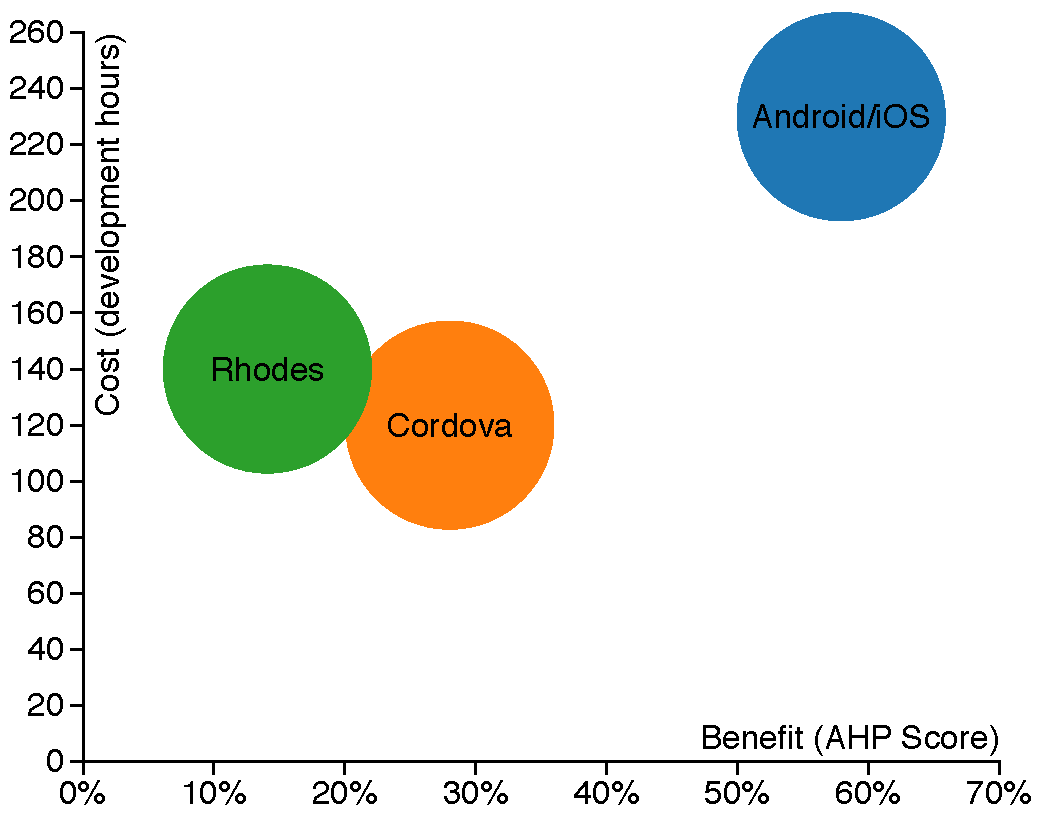
\includegraphics[width=0.7\textwidth]{figs/benefit-cost.pdf}
    \caption{Visual representation of the cost-benefit analysis. The benefits are indicated on the horizontal axis. The cost of the project is represented by the development time on the vertical axis.}
    \label{fig:cost-benefit}
\end{figure}

It is important to mention that adding an additional platform to the native portfolio will increase the development time (and cost) by half, whereas additional platforms can be added at virtually no cost when developing mobile web applications with Cordova. In case a third platform has to be supported, Cordova application will have better value-for-money.
